\section{Image Labeling}

Part of the dataset is manually annotated to provide ground truth tip locations, leaf segmentation results and leaf consistency overtime. 
Tip locations are saved in TXT file \textcolor{red}{(TBD)}.
Leaf segmentation results are stored in PNG images with one color for each leaf.
The same color is used to represent the same leaf over a sequence of frames. 

We use RGB images for labeling because of better visualization. 
All plants are cropped out from the background and saved as JPG files. 
For Arabidopsis images, we label four frames each day. 
While for bean images, we label seven frames each day because of faster leaf movement. 
We develop a Matlab GUI interface for leaf labeling, as shown in Fig~\ref{fig:label}.
A user can open an image to label the two tips and annotate each leaf. 
The results will be automatically saved once a user goes to label the next image. 
This GUI is used to annotate leaves in each frame. 
For consistent annotation of the same leaf over time, we use the labeled results of each frame to find the correspondence according to leaf centers. 
Incorrect correspondence will be manually corrected. 

\begin{figure}[h]
\centering
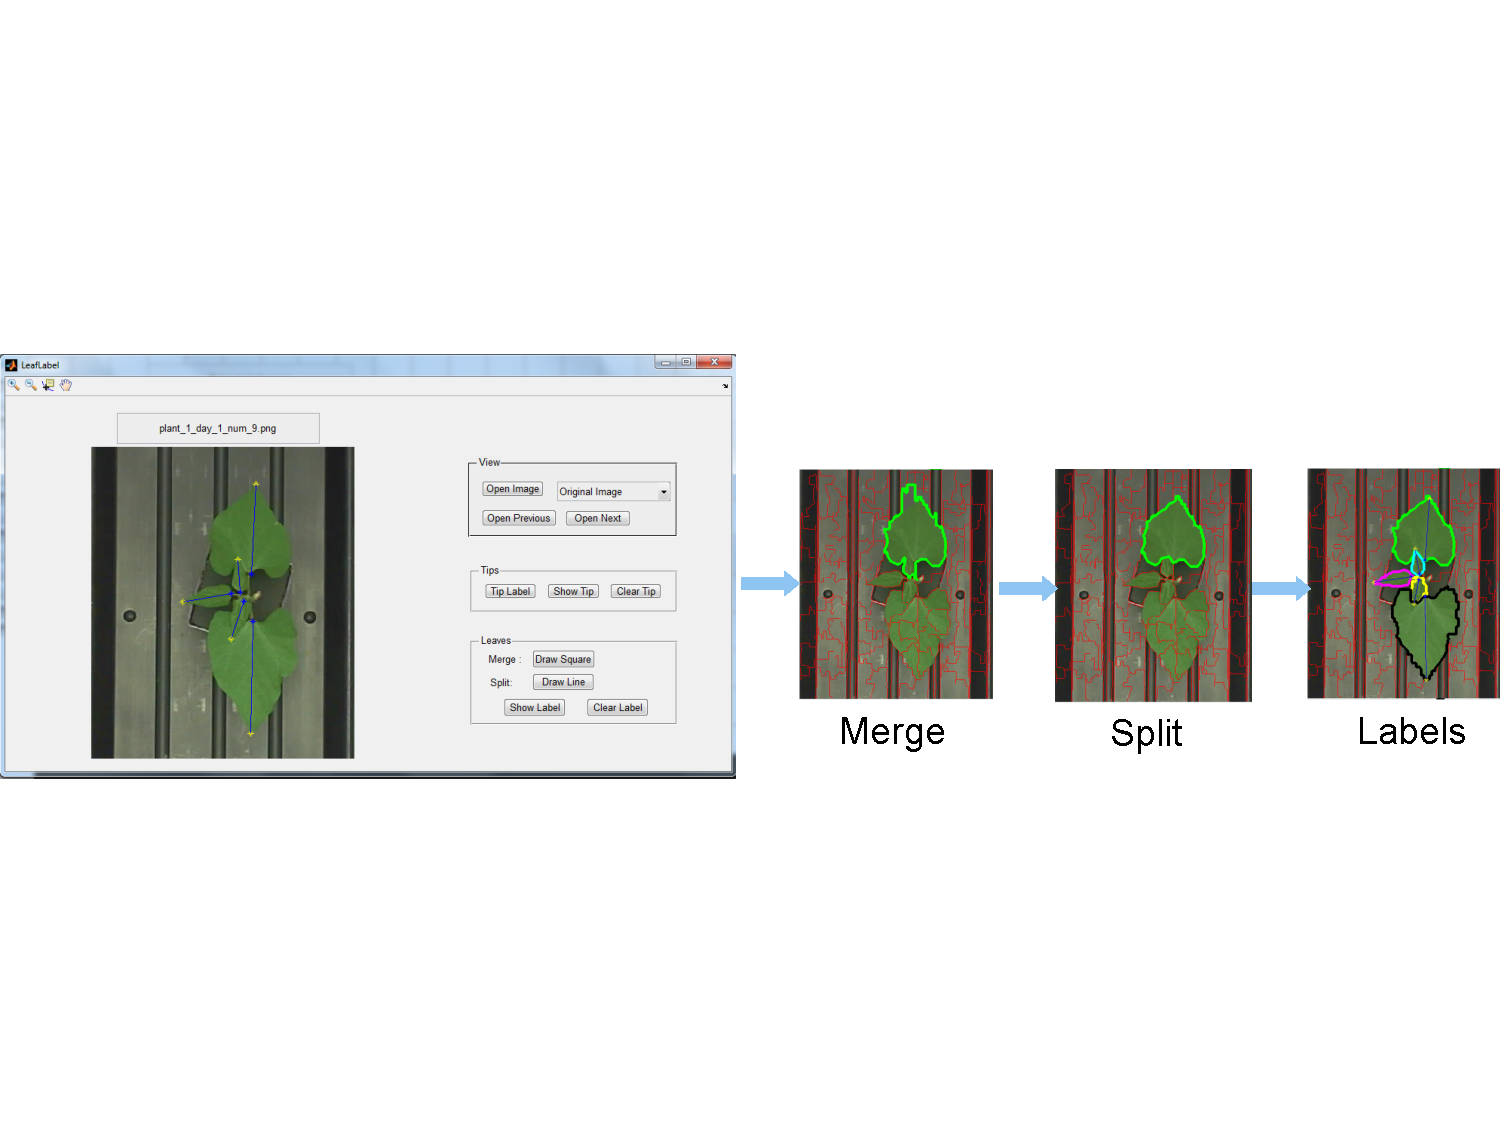
\includegraphics[width=.98\textwidth]{figure/labeling}\\
\caption{Leaf labeling process, including tip labels and leaf annotation.}
\label{fig:label}
\end{figure}

Tip label is implemented by clicking pairs of points on the image. 
The outer tip is always clicked before the inner tip. 
A line connecting each pair of tips will be shown immediately for visualization. 
Inaccurate labels can be deleted and relabeled. 

For leaf annotation, we use the idea of merging and splitting super pixels. 
There are six different numbers of super pixels: $100$, $200$, $300$, $500$, $800$, $1000$. 
The user can specify which level to use depending on how well the super pixels can separate the leaves from the background. 
Because one leaf can be covered by several super pixels and one super pixel can across two leaves or the foreground and background. 
We allow merging and splitting super pixels. 
Merging is implemented by drawing a rectangle on the image. 
Every super pixel overlapping with this rectangle will be merged together. 
Splitting is implemented by drawing a line separating a leaf from the background or from another leaf. 

As shown in Fig.~\ref{fig:label}, several super pixels that covers one leaf are first merged together to form a large super pixel. 
Since the top part of the super pixel covers some of the background and the bottom part covers another small leaf, two lines are drawn on this super pixel to split it. 
The leaf boundary is overlaid on the image for better visualization to guide the next action. 
This process continues until all leaves have been annotated. 















